\documentclass[journal,10pt,letterpaper]{IEEEtran}
\usepackage[T1]{fontenc}
\usepackage[utf8]{inputenc}
\usepackage{amsmath,amssymb,graphicx,booktabs,tabularx,array}
\usepackage[table]{xcolor}
\usepackage[most]{tcolorbox}
\usepackage{microtype}
\usepackage{needspace}
\usepackage[hidelinks]{hyperref}
\usepackage{url}
\definecolor{pendingbg}{HTML}{FFF2CC}
\definecolor{pendingborder}{HTML}{BF9000}
\DeclareUnicodeCharacter{03B1}{\ensuremath{\alpha}}
\DeclareUnicodeCharacter{03B3}{\ensuremath{\gamma}}
\DeclareUnicodeCharacter{03C1}{\ensuremath{\rho}}
\DeclareUnicodeCharacter{03B5}{\ensuremath{\epsilon}}
\DeclareUnicodeCharacter{03C3}{\ensuremath{\sigma}}
\DeclareUnicodeCharacter{03BC}{\ensuremath{\mu}}
\DeclareUnicodeCharacter{0394}{\ensuremath{\Delta}}
\DeclareUnicodeCharacter{2190}{\ensuremath{\leftarrow}}
\DeclareUnicodeCharacter{2212}{\ensuremath{-}}
\DeclareUnicodeCharacter{0307}{\ensuremath{\dot{\phantom{x}}}}
\providecommand{\tightlist}{\setlength{\itemsep}{0pt}\setlength{\parskip}{0pt}}
\setlength{\emergencystretch}{1em}
\begin{document}

\title{GECO: Separating Delivery Evidence and Stop Authority in an Insulin-Pump Simulation Study}
\author{Author information pending the research team}
\maketitle
\begin{abstract}Monitoring an automated insulin-delivery system requires distinguishing a permitted command from delivered fluid and accounting for the delivery withheld by containment. This paper evaluates GECO, an offline research method that separates requests, authorization, simulated emission, measurement reports and stop authority. A corrected causal estimator and forecast selector were evaluated on previously exposed internal test segments from 31 participants, comprising 77,110 matched 30-minute forecast pairs. Validation selected trend forecasting for 30 participants and persistence for one; selected forecasting reduced mean participant RMSE by 4.14 mg/dL relative to persistence, while the mechanistic forecast was worse for 28 participants. A prespecified comparison completed 4,608 fixed-request simulations and 576 feedback/stop sensitivity simulations with no execution failures. Under matched authority, the fuller detector increased stuck-on excess relative to a simpler detector by 0.137 research U in the original plant family and 0.085 research U in a Hovorka implementation. Overall, 2,108 main runs violated the physiological-domain screen, including 44 of 48 clean Hovorka runs per arm. A subsequent 2,048-run exploratory fasting supplement passed the declared domain screen but retained nuisance stops and condition-dependent excess/deficit tradeoffs. These findings support neither universal detector superiority nor clinical benefit. The contribution is a reproducible comparison that exposes containment tradeoffs and model limits, together with a proposed uncertainty-aware water/saline measurement protocol. IIT Patna physical measurements remain pending.\end{abstract}
\begin{IEEEkeywords}automated insulin delivery, runtime monitoring, delivery measurement, digital twin, causal forecasting, fault containment, simulation, metrology.\end{IEEEkeywords}
\section{Introduction}

An automated insulin-delivery loop converts glucose observations into
pump commands. A command expresses an intended action; authorization
determines whether that action is permitted; an endpoint acknowledgment
reports message acceptance; and fluid delivery is a physical
consequence. These quantities can diverge. An occluded outlet may
deliver nothing after a valid command, while a malfunctioning actuator
may emit more than authorized. A measurement report introduces another
boundary because an instrument indication can be noisy, delayed or
replaced in communication. A monitor must state which quantity it
observes before its alarm can be interpreted.

Response introduces a second problem. Stopping future powered delivery
can contain excess, but it also withholds subsequent requested delivery.
A longer latch may improve one excess metric while increasing deficit,
interruption or recovery time. Comparing a monitor that can stop an
actuator with one that cannot conflates evidence quality with response
authority. GECO investigates these distinctions through a
shared-authority comparison and reports excess and deficit separately.

The relevant foundations already exist. GlucOS implements a BioKernel
reference monitor and layered safeguards for automated insulin delivery
\cite{R01}. KnowSafe studies prediction and mitigation of
artificial-pancreas hazards, including consequences of intervention
\cite{R02}. Pump calibration and Kalman-assisted delivery metrology also
predate this work \cite{R03,R04}. GECO therefore makes no claim to
invent a reference monitor, digital twin, insulin-pump measurement
method or Kalman filter. Its contribution is a reproducible,
outcome-neutral evaluation of an explicit evidence/authority model,
including cases where a more elaborate detector performs worse.

Three questions organize the study. First, does the retained mechanistic
estimator provide useful causal forecast evidence compared with simple
baselines on supplied records? Second, how do detector and recovery
policies change emitted delivery when requests and response authority
are matched? Third, what measurements are still needed before a physical
rig can supply a defensible virtual-patient input? The answers are
separated because forecasting, fault discrimination, containment and
physical measurement are different claims.

The completed contributions are: a corrected causal estimation and
forecast-selection implementation with an internal retrospective
evaluation; a prespecified simulation comparison using two structurally
different plant families, matched exogenous inputs and complete outcome
records; and an acquisition/reconstruction protocol that makes the
missing physical evidence explicit. The main detector comparison is
negative or mixed. The second plant also exposes substantial domain
violations. These are central findings, not exclusions from the result
denominator.

\section{Prior Work and Scope}

GlucOS places runtime checks around automated insulin delivery, while
KnowSafe combines knowledge and data for hazard mitigation
\cite{R01,R02}. Both limit any broad claim that an additional safety
layer or predictive monitor is new. The present comparison asks a
narrower question about authorization under separately represented
delivery observations. It does not reproduce either system, execute a
head-to-head benchmark against them, or show that their stated
assumptions are invalid. Their experiments and threat models should not
be replaced with the abstractions used here.

Bissig and colleagues examine insulin-pump calibration through discrete
doses and their timing \cite{R03}. Girardot and colleagues describe
Kalman-assisted pump-accuracy assessment \cite{R04}. These establish
that delivery measurement requires more than command accounting. GECO
borrows no numerical accuracy benchmark from those papers. Its simulated
balance is an assumed observation model, and the conceptual bench
remains unmeasured. JCGM 100 provides a framework for defining the
measurand, corrections and uncertainty; it does not certify this
apparatus \cite{R09}.

Hovorka and colleagues provide the compartment equations and parameter
means used for the independent plant implementation \cite{R05}. The
original fasting-control study does not validate arbitrary
meal/controller regimes in a derivative simulator. The UVA/Padova
simulator has a separate model lineage and documented refinements
\cite{R08}; it was not executed here, and no validation or regulatory
history transfers to GECO. Unscented filtering is established
\cite{R06}, and personalized plasma-insulin estimation with Hovorka
dynamics and a UKF has been studied \cite{R07}. GECO retains an extended
Kalman implementation and reports no EKF--UKF experiment or universal
filter ranking.

The literature review was bounded, with primary-source identities and
claim locators recorded. Selected full-text sections supported GlucOS,
KnowSafe, Hovorka and personalized-estimation comparisons.
Pump-metrology access was partial or abstract-only, and the foundational
UKF reference was checked bibliographically rather than reviewed in full
during this update. These limits prevent unsupported performance
comparisons. The distinct contribution is the executed matched study and
its reproducible limitations, rather than an exhaustive novelty claim.

\section{Quantities, Authority and Fault Model}

At five-minute interval k, let \(r_k\) denote the requested amount and
\(a_k\) the authorized amount, in research U. Let \(m_k\) be latent
emitted mass, \(b_k\) the local cumulative balance indication, and
\(d_k\) the received interval-mass report. The simulator converts
\(m_k\) to plant input using the declared convention γ = 0.1005
g/research U. This mapping represents an offline water/saline
abstraction. It is not a measured insulin concentration or a clinical
dosing specification.

The main experiment generates one clean feedback request tape for each
synthetic parameter unit and exogenous seed. Every paired arm receives
that same \(r_k\), meal sequence and noise arrays. A policy may inhibit
or cap \(a_k\); a simulated fault changes \(m_k\); the measurement
channel produces \(b_k\) and \(d_k\). Only \(m_k\)/γ drives the
physiological plant. Neither noisy mass differences nor the potentially
replaced network report can alter that evaluator input. The monitor
receives reported CGM, available mass observations and prior authorized
inputs, without evaluator glucose, emitted mass or fault-end labels.

\begin{table}[!t]
\centering
\caption{Evidence quantities and access boundaries}
\label{tab:1}
\small
\setlength{\tabcolsep}{3pt}
\renewcommand{\arraystretch}{1.17}
\begin{tabularx}{\linewidth}{>{\raggedright\arraybackslash}p{0.29\linewidth}>{\raggedright\arraybackslash}p{0.64\linewidth}}
\toprule
\textbf{Quantity} & \textbf{Meaning and access} \\
\midrule
Request \(r_k\) & Clean controller intent shared across main-comparison arms \\
Authorization \(a_k\) & Amount permitted by the detector/recovery policy \\
Emission \(m_k\) & Latent actuator output; simulator and evaluator only \\
Local indication \(b_k\) & Quantized, noisy cumulative observation available to every local guard \\
Received report \(d_k\) & Interval report; may be replaced in one coordinated condition \\
Reported CGM \(y_k\) & Sensor observation; may be biased or missing \\
Physical reconstruction & Future validated estimate with uncertainty; not available in this study \\
\bottomrule
\end{tabularx}
\end{table}

The controller uses a unit-specific equilibrium basal assumed known at
setup. Above 150 mg/dL it adds 0.0025 research U per mg/dL above that
threshold; it suspends below 100 mg/dL or a forecast below 90 mg/dL,
with a 0.3 research-U interval cap. The 120 mg/dL value defines
equilibrium initialization, not the implemented correction threshold.
Its configuration is common across arms. Knowing equilibrium basal is a
simulation setup assumption, not proof that the transferred twin
identifies an individual physiology.

Eight conditions are evaluated: clean; a twofold powered actuator-input
multiplier before quantization, gain, noise and offset; zero delivery
from occlusion; a nominal stuck-on addition of 0.25 research U, scaled
by 1.015 to 0.25375 emitted research U per powered interval; CGM bias of
+40 mg/dL; missing CGM; the twofold input multiplier with +25 mg/dL CGM
bias; and the latter combination with the received mass report replaced
by authorized mass. Perturbations occupy intervals 144--167,
corresponding to hours 12--14. They are numerical fault/compromise
abstractions. No radio, packet, credential, firmware or live-device
attack was performed.

The report-replacement condition retains the unmodified local balance
guard in every arm. It consequently evaluates a specified remaining
observation path, not successful detection after all physical witnesses
are compromised. If two physical histories induce identical available
observations and authority states, the practical monitor receives no
additional truth from the simulation. The separately labelled oracle
knows the physical-fault window and inhibits delivery during it; it is
an explanatory privileged reference, not an achievable detector.

\section{Causal Estimation and Forecast Evidence}

\subsection{State, timing and covariance}

The retained five-state research model contains plasma glucose G, remote
insulin action X, insulin state I, gut carbohydrate Q and interstitial
glucose \(G_i\):

\[\begin{gathered}
\dot G=e_{gp}-p_1G-X\max(G,30)+k_c k_aQ,\\
\dot X=-p_2X+p_3(I-I_b),
\end{gathered}\]

\[\begin{gathered}
\dot I=-k_iI+k_u u,\\ \dot Q=-k_aQ+c,\\
\dot G_i=(G-G_i)/\tau_i. 
\end{gathered}\tag{1}\]

Here u is research U/min and c is carbohydrate g/min. Five one-minute
Euler substeps advance each observation interval. Numerical clamps
retain G and \(G_i\) within 20--600 mg/dL, X at or above −\(p_1\)/2, and
I and Q nonnegative. The transition Jacobian includes these piecewise
operations; active clamp rows have zero derivative. These are numerical
rules, not independently validated biological boundaries.

The update at time k advances the model using \(a_{k-1}\) and
carbohydrate input from the previous interval, then assimilates the
current CGM. Initialization uses the first current observation and a
frozen basal steady-state approximation. Initializing and reset
observations do not generate valid prediction errors. Missing data break
trend/AR history, and a return after 60 minutes missing resets the
filter. Hidden insulin and gut history are approximated on reset, which
remains a limitation.

For \(H=[0,0,0,0,1]\), the nominal innovation variance and gain are
\(s_k=HP_k^-H^T+R_k\) and \(K_k=P_k^-H^T/s_k\). Covariance uses the
Joseph form \cite{R13}:

\[
P_k^+=(I-K_kH)P_k^-(I-K_kH)^T+K_kR_kK_k^T. \tag{2}
\]

The same nominal \(R_k\) enters gain and covariance. Its base value is
81 \((\mathrm{mg/dL})^2\), increased according to predicted low/high
CGM; process-noise values remain declared heuristic settings.
Symmetrization and finite/eigenvalue checks separate negligible roundoff
projection from material covariance failure, which triggers a recorded
reset. Numerical tests establish implementation properties under their
fixtures; they do not establish clinical estimation accuracy.

A fitted scale α affects anomaly normalization only:
\(z_k^{\mathrm{raw}}=(y_k-H\hat x_k^-)/\sqrt{\alpha s_k}\). It does not
change gain, state or covariance. Adjacent valid fit innovations
estimate ρ, clipped to {[}0,0.98{]}, and the monitoring statistic is

\[
z_k=(z_k^{raw}-\rho z_{k-1}^{raw})/\sqrt{1-\rho^2}. \tag{3}
\]

Initializing/reset observations remain invalid; the first valid
innovation after a gap/reset is unwhitened. Let \(w_k^0\) be the
AR-whitened nominal innovation before α scaling. Then
\(\alpha=\max(10^{-6},[q_{0.95}(|w^0|)/1.96]^2)\). This calibration does
not make observations independent or Gaussian; empirical coverage and
alarm burden are reported separately.

\subsection{Fitting, selection and internal evaluation}

Supplied records were associated with HUPA-UCM version 1 and D1NAMO
version 1.2.0 \cite{R14,R15}. The source repositories identify CC BY 4.0
and CC BY-SA 4.0, respectively. This analysis used the supplied local
records and loader transformations, without obtaining new participant
data. HUPA preprocessing can include interpolation, while D1NAMO
carbohydrate conversion from calories and slow-insulin allocation are
proxies rather than verified administration records. Forecasts are
causal with respect to the supplied sample order, but upstream offline
interpolation may not reproduce observations available in real time.
Absence of future-array access does not establish that every
preprocessed input was generated causally.

Chronological splits were floor(0.5N), floor(0.75N) and the remaining
segment. Eligibility required at least 288 fit slots and 144 tune/test
slots, at least 50\% supplied finite CGM in each segment, and 50
forecast pairs after a 36-slot warmup. Four
quantities---\(e_{gp}\)/\(p_1\), \(p_1\), \(k_c\) and \(p_3\)---were
fitted within prespecified log bounds using two deterministic
least-squares starts. The objective used causal 30-minute mechanistic
residuals at every sixth eligible fit origin. Basal hold came from the
fit-window median supplied basal; no clinical sensitivity-rule prior
constrained \(p_3\). Optimizer convergence does not establish unique
physiological identification.

Every eligible origin produced three predictions on the same
target/mask. The mechanistic forecast repeated frozen basal and assumed
no future meals; persistence retained current CGM; trend used up to four
consecutive observations, an ordinary least-squares slope clipped to ±3
mg/dL/min, and 0.5 damping over 30 minutes. Future observations, meals
and insulin records were unavailable to prediction. This conservative
timing may leave contemporaneous information unused, but it is common to
all policies. Lowest tune RMSE selected the runtime policy, with
persistence preferred in ties.

The selected forecast's fit errors ε provided the scale
\(\sigma_6=\max(1,q_{0.95}(|\varepsilon|)/1.96)\) mg/dL. Each physiology
channel received half a one-episode/day tune budget over thresholds from
4 to 128 in increments of 0.5. The alarm union was evaluated separately;
meeting the tune budget did not guarantee test performance.
Configuration was frozen before a separate test invocation. These
segments had been exposed in earlier project work, so the final
evaluation is an internal chronological test, not new external
validation. Participant-level paired bootstrap intervals used 10,000
resamples, with equal participant weighting.

\section{Shared-Authority Monitoring and Recovery}

For authorized amount \(a_k\), the expected mass accounts for simulated
quantization and offset:

\[
\mu(a_k)=1.015\gamma\,\mathrm{round}(200a_k)/200+0.0015\quad(a_k>0), \tag{4}
\]

and μ(0)=0. Actual nominal emission has 0.0008 g Gaussian noise on
positive quantized delivery and is bounded below by zero. The cumulative
balance uses the median of five observations with 0.003 g Gaussian
noise, then 0.01 g quantization. Signed interval differences are
retained; they are not rectified into simulated plant input.

The simple score is \(|d_k-\mu(a_k)|/\sigma_m\). The fuller detector
maintains delivery and physiology two-sided CUSUMs. With standardized
input v, positive and negative accumulators update as
\(C^+\leftarrow\max(0,C^++\mathrm{clip}(v,-6,6)-0.5)\) and
\(C^-\leftarrow\max(0,C^--\mathrm{clip}(v,-6,6)-0.5)\);
\(C=\max(C^+,C^-)\). The physiology group selects the signed member with
greatest absolute magnitude from the standardized innovation and due
causal forecast residual. Both are transformations of the same CGM
stream and count as one group. The fuller score is

\[
S_k=\max(C_{m,k},\sqrt{C_{m,k}C_{g,k}}). \tag{5}
\]

Absent a current valid physiology input, only the delivery term is used.
This heuristic score is not a calibrated probability. Full versus simple
changes both temporal aggregation and physiology corroboration; it
cannot isolate the physiology channel's incremental contribution.
Section VII-E examines that component-policy question in a narrower
post-primary fasting supplement.

Both detectors share a 0.3 research-U cap, a local interval excess
margin of 0.03 g, a 12-interval cumulative excess margin of 0.05 g, and
a 1.05 authorized-mass factor. Six consecutive missing CGM samples also
trigger containment. Separate thresholds strictly exceeded the maximum
warmup-excluded statistic over 32 clean calibration runs: 7.44947 for
full and 3.10096 for simple. Zero empirical statistical containment in
these tuning runs is a finite-sample fitting result.

The six arms are full/manual, full/supervised, simple/manual,
simple/supervised, sham/manual and oracle. Sham disables the statistical
detector but retains local-budget and sensor-quality rules. All
practical arms use identical local observations and stop authority. The
study adapter imports the corrected estimator/controller components; it
does not execute the complete legacy protocol, attestation or
security-kernel stack.

Containment is observed at the end of an interval and inhibits
subsequent powered delivery. Already emitted mass cannot be removed. A
fixed operator authorization occurs every 120 minutes, independently of
fault labels. Reset requires at least 30 minutes since the trip interval
ended, six quiet local observations with absolute net change at most
0.01 g, and available current CGM. Manual emulation clears the latch.
Supervised emulation enters three verification intervals capped at
min(\(r_k\),0.08), requiring positive expected delivery and aggregate
measured mass within 0.012 g of expectation, then six similarly capped
probation intervals. Missing CGM during verification, or failure of its
aggregate check, relatches. No missed amount is accumulated for
catch-up.

\begin{quote}\footnotesize\ttfamily\raggedright
For each interval k:\\
Read current reported CGM; update twin with prior authorized inputs.\\
Obtain shared clean request, or own feedback request in sensitivity runs.\\
If a scheduled operator slot satisfies cooldown and observed quiet rules:\\
clear latch manually, or enter bounded verification.\\
Authorize according to RUN / LATCHED / VERIFY / PROBATION state.\\
Simulate emission, local indication and received report separately.\\
Update delivery/physiology evidence and shared local/quality rules.\\
At interval end, latch on any applicable trigger.\\
Advance evaluator plant from emitted mass only; preserve complete record.\\
\end{quote}

Quiet observations can be misleading, and zero-demand verification
cannot confirm delivery. Operator availability and the selected schedule
are assumptions. These rules emulate supervision; they are not evidence
of autonomous, safe restart.

\section{Simulation Design and Analysis}

Each plant family contains eight calibration and 24 locked test
parameter units, with two repeated seeds per unit. The original family
uses (1), while the second is a GECO implementation of Hovorka equations
1--7 and Tables 1--2 \cite{R05}. The Hovorka plant has accessible/remote
glucose \(Q_1\),\(Q_2\), two subcutaneous insulin states
\(S_1\),\(S_2\), plasma insulin I, three insulin-action states
\(x_1\),\(x_2\),\(x_3\), and two gut transit states. Its glucose
dynamics are

\[\begin{gathered}\dot Q_1=-F_{01}^c-x_1Q_1+k_{12}Q_2-F_R+U_G+EGP_0(1-x_3),\\
\dot Q_2=x_1Q_1-(k_{12}+x_2)Q_2,\qquad G=Q_1/V_G. 
\end{gathered}\tag{6}\]

Insulin actions follow \(\dot x_i=k_{ai}(S_{Ii}I-x_i)\); subcutaneous
insulin forms a two-stage transit chain. The two gut states implement
the published meal impulse response for interval-constant input. Q is in
mmol, S in mU, I in mU/L, \(x_1\)/\(x_2\) in \(\mathrm{min}^{-1}\) and
\(x_3\) dimensionless. Conversions are 1000 mU/U, 0.1801559 g
glucose-equivalent carbohydrate/mmol and 18.01559 mg/dL per mmol/L
glucose. The original Table 2 sensitivity means, visually verified in
the primary paper, are \(51.2\times10^{-4}\) and \(8.2\times10^{-4}\)
\(\mathrm{min}^{-1}\) per mU/L and \(520\times10^{-4}\) per mU/L.

A nonnegative fasting equilibrium at 120 mg/dL supplies basal
initialization; one-minute RK4 substeps integrate Hovorka dynamics. A
nine-minute sensor lag is a separately disclosed extension. Body weight
and family-specific parameter factors are synthetic engineering
variations, not draws from a fitted patient distribution. Some
original-family fields do not affect that model, so perturbation
dimensions are not identical across families. The pooled twin uses
coordinate-median fresh calibration parameters and the modal selected
forecast policy, which was trend; it is a transfer configuration rather
than a participant-specific synthetic twin. Unlike real-data
initialization from current CGM, the synthetic twin resets to 120 mg/dL
and does not assimilate the first sample.

The main matrix is 48 test units × 2 seeds × 8 conditions × 6 arms =
4,608 runs. Each contains 576 intervals, or 48 hours. Meals occur three
times daily with paired timing/amplitude variation. CGM, pump and
balance draws are paired by family/unit/seed. Statistical warmup is
three hours. The independent unit is the synthetic parameter vector;
seeds are repeated realizations within it.

The 576-run sensitivity uses the first six locked units per family, both
seeds, four conditions and full/simple supervised policies. Each arm
generates feedback-dependent requests and uses an arm/stop-matched clean
reference. Three stop assumptions are evaluated: inhibit subsequent
powered delivery; allow one additional five-minute powered interval; or
add a residual tail of 0.02 research U for three intervals. These
assumptions are not measured rig dynamics, and this feedback estimand is
distinct from the main fixed-request comparison.

For actual emitted amounts \(e_k=m_k/\gamma\) and paired clean reference
\(e_k^0\), delivery outcomes are

\[\begin{gathered}
E^+=\sum_k\max(e_k-e_k^0,0),\\
E^-=\sum_k\max(e_k^0-e_k,0),\\
E^{net}=\sum_k(e_k-e_k^0). 
\end{gathered}\tag{7}\]

An interruption requires positive request and zero emission. Commanded
latch exposure uses state before emission, avoiding an interval-boundary
shift. Recovery is the first six-interval post-fault window without a
latch and with authorization at least 95\% of request, with some
positive demand. Its onset and confirmation 30 minutes later are
distinct; this measures authorization restoration, not physical or
clinical recovery. Censoring is retained. First-trip latency is relative
to scheduled onset and may be negative for an earlier nuisance trip.

All plant-domain failures remain in the denominator. In Hovorka,
\(x_3\)\textgreater1 makes the published endogenous-production term
negative; the equation is retained and separately flagged.
Negative/nonfinite or other screened state violations are also recorded.
Original-family plasma/interstitial/action boundary counts expose
clipping beyond its plasma-domain screen. Neither a passing screen nor
numerical boundedness establishes physiological validity. Glucose-band
results on invalid trajectories are mathematical summaries.

Paired differences average the two seeds within each parameter unit,
then use 4,096 percentile bootstrap resamples of units. Families,
conditions, recovery policies and stop assumptions remain separate.
Intervals describe this synthetic design; they are not patient
uncertainty or multiplicity-adjusted superiority tests. Initial
specification and three pre-outcome amendments preserve timing/domain
corrections. Sources and configuration were frozen before execution,
with complete attempts, failures and per-sample traces retained.

\section{Results}

\subsection{Internal forecast evaluation}

Of 34 supplied participant records, 31 were evaluated: 24 HUPA and seven
D1NAMO. D1NAMO 003 and 009 were excluded for insufficient
length/coverage, and HUPA0017P failed input validation because supplied
bolus values included −1 and −3 U. They were not silently repaired. An
earlier packaging/import-order failure was retained as a separate
attempt; the final frozen fit and test were separate invocations.

The 31 evaluations contained 77,110 matched forecast-origin/target
pairs. HUPA0027P contributed 41,285 pairs, making pooled-pair accuracy
strongly duration-weighted; equal-participant summaries were therefore
used. Validation selected trend for 30 participants and persistence for
one, with no mechanistic selection. The selected policy improved on
persistence for 30 participants and tied for one. The mechanistic
forecast was worse than persistence for 28 of 31 participants.

\begin{table*}[!t]
\centering
\caption{Internal participant forecast evaluation}
\label{tab:2}
\small
\setlength{\tabcolsep}{3pt}
\renewcommand{\arraystretch}{1.17}
\begin{tabularx}{\linewidth}{>{\raggedright\arraybackslash}p{0.24\linewidth}>{\raggedright\arraybackslash}p{0.26\linewidth}>{\raggedright\arraybackslash}p{0.43\linewidth}}
\toprule
\textbf{Forecast} & \textbf{Median participant test RMSE (mg/dL)} & \textbf{Mean paired RMSE minus persistence, 95\% interval (mg/dL)} \\
\midrule
Mechanistic & 25.77 & +3.73 {[}2.56, 4.91{]} \\
Persistence & 22.56 & Reference \\
Damped trend & 17.83 & −4.00 {[}−4.95, −3.03{]} \\
Tune-selected policy & 17.59 & −4.14 {[}−5.02, −3.33{]} \\
\bottomrule
\end{tabularx}
\end{table*}

Median empirical nominal-95\% coverage was 96.05\% for innovations and
95.82\% for selected forecasts, with participant ranges 86.12--98.73\%
and 87.50--98.92\%. Near-nominal median coverage obscures participant
variation. Thirteen participants exceeded one union alarm/day on test,
with a maximum of 12/day; the median was 0.814/day. Twenty-four fits
were near at least one parameter bound. Thus validation-selected causal
forecasting improved this internal prediction comparison, but neither
reliable physiological identification nor a uniformly low monitoring
burden was demonstrated.

\subsection{Completed comparison and model-domain findings}

\begin{figure*}[!t]\centering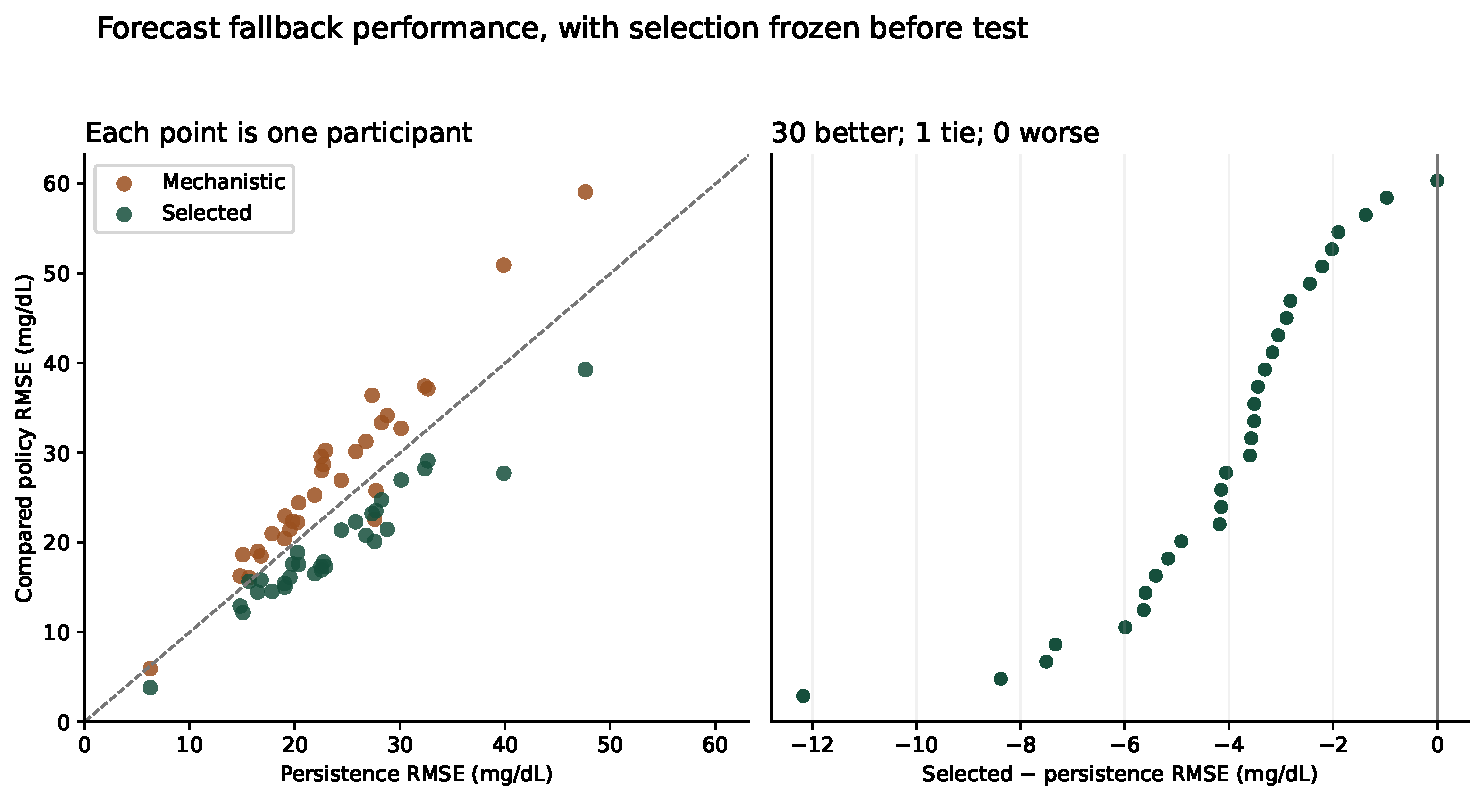
\includegraphics[width=.88\textwidth]{paper_figures/Figure1.pdf}\caption{Participant-level internal forecast comparison. The selected policy was chosen on tune data; each plotted point is one of 31 evaluated participants. Previously exposed test segments and upstream preprocessing limit prospective interpretation.}\label{fig:1}\end{figure*}

\begin{figure*}[!t]\centering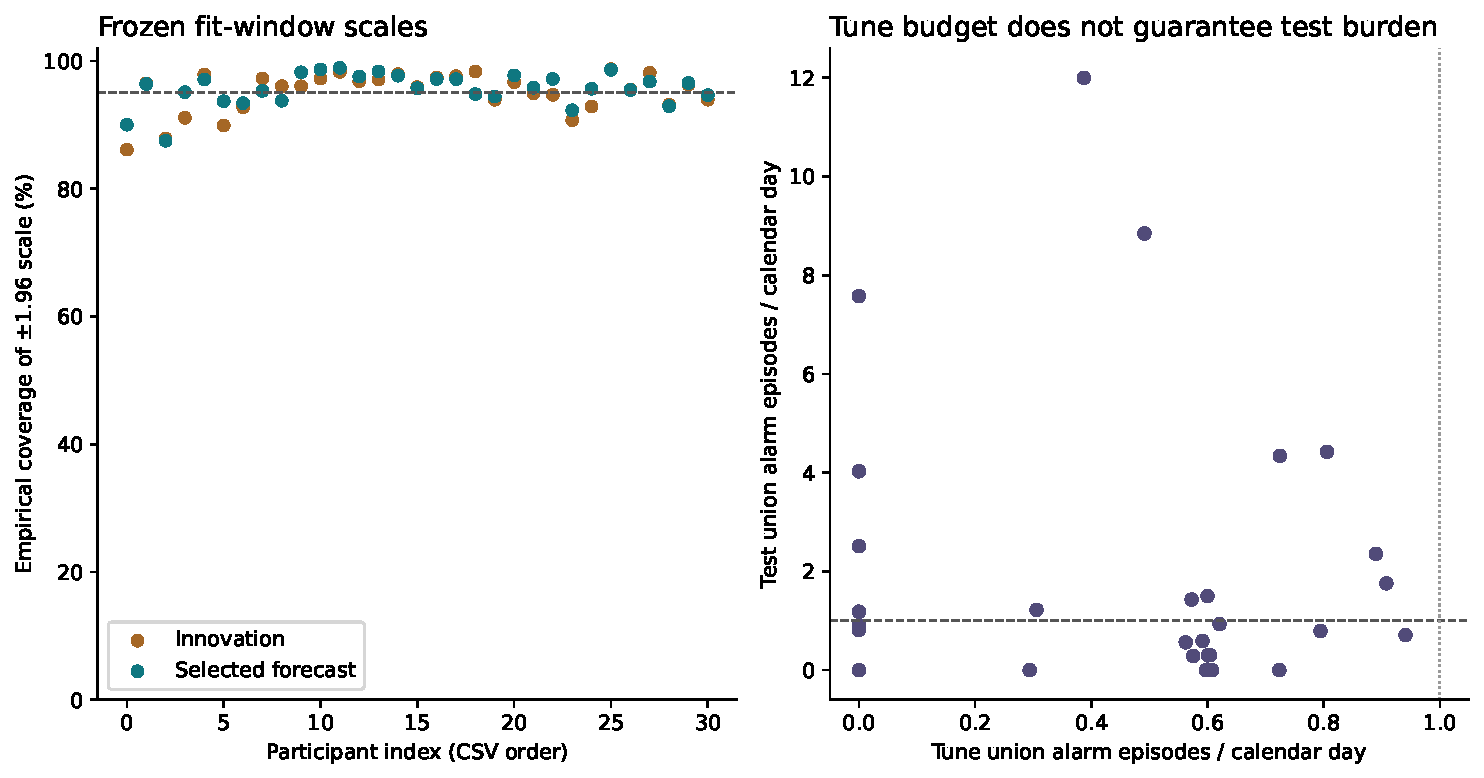
\includegraphics[width=.92\textwidth]{paper_figures/Figure2.pdf}\caption{Empirical test residual coverage and tune-to-test alarm burden. Near-nominal median coverage does not imply uniform participant coverage or a preserved alarm budget; 13 of 31 participants exceeded one test union alarm per day.}\label{fig:2}\end{figure*}

All 5,184 assigned simulations completed: 4,608 main and 576
feedback/stop runs, with zero final execution failures. Complete traces
comprise 2,985,984 samples. No out-of-domain run was removed. Of the
4,608 main runs, 2,108 failed at least one physiological-domain screen;
all were in the Hovorka family. In the clean condition, 44/48 Hovorka
runs per arm had domain violations and negative endogenous production.
The Hovorka main traces contained 138,103 invalid samples of 1,327,104,
and 579 runs reached negative glucose, with a minimum of −20.91 mg/dL.
This occurs before interpreting a fault response and limits the family
as evidence of physiological robustness.

The original family had zero main runs failing its plasma-domain screen,
but clipping still mattered: clean traces contained 100 remote-action
boundary samples per arm. Across all original-family main runs there
were 34,731 such samples. Absence of its coarse validity flag therefore
cannot be described as independent model validation. Hovorka had 133,394
negative-EGP samples across main runs. No clinical glucose-benefit claim
is made from either family.

Locked clean original-family runs had no trips in any arm. Hovorka clean
full/manual and full/supervised each tripped in 2/48 runs, whereas
simple, sham and oracle had none. These full-arm latches did not produce
a nonzero aggregate delivery deficit relative to the reference under the
requested tapes; a trip count and a withheld-delivery outcome are
different quantities. The same benign calibration criterion therefore
did not imply identical locked clean containment burden.

\subsection{Matched delivery and recovery tradeoffs}

\begin{table*}[!t]
\centering
\caption{Full/supervised minus simple/supervised delivery differences. Mean paired research U [95\% parameter-unit interval]; 24 units and 48 paired seed-runs per row.}
\label{tab:3}
\small
\setlength{\tabcolsep}{3pt}
\renewcommand{\arraystretch}{1.17}
\begin{tabularx}{\linewidth}{>{\raggedright\arraybackslash}p{0.12\linewidth}>{\raggedright\arraybackslash}p{0.29\linewidth}>{\raggedright\arraybackslash}p{0.26\linewidth}>{\raggedright\arraybackslash}p{0.26\linewidth}}
\toprule
\textbf{Plant} & \textbf{Condition} & \textbf{Excess difference (U)} & \textbf{Deficit difference (U)} \\
\midrule
Original & Clean & +0.000 {[}+0.000,+0.000{]} & +0.000 {[}+0.000,+0.000{]} \\
Original & 2× actuator input & +0.010 {[}+0.000,+0.025{]} & -0.011 {[}-0.028,+0.000{]} \\
Original & Occlusion & +0.000 {[}+0.000,+0.000{]} & -0.047 {[}-0.163,+0.015{]} \\
Original & Stuck-on addition & +0.137 {[}+0.100,+0.174{]} & -0.281 {[}-0.567,-0.042{]} \\
Original & CGM +40 & +0.000 {[}+0.000,+0.000{]} & +0.000 {[}+0.000,+0.000{]} \\
Original & CGM missing & +0.000 {[}+0.000,+0.000{]} & +0.000 {[}+0.000,+0.000{]} \\
Original & 2× input + CGM +25 & +0.010 {[}+0.000,+0.023{]} & -0.011 {[}-0.027,+0.000{]} \\
Original & 2× input + bias + report replacement & +0.000 {[}+0.000,+0.000{]} & +0.000 {[}+0.000,+0.000{]} \\
Hovorka & Clean & +0.000 {[}+0.000,+0.000{]} & +0.000 {[}+0.000,+0.000{]} \\
Hovorka & 2× actuator input & -0.003 {[}-0.019,+0.013{]} & +0.206 {[}+0.000,+0.479{]} \\
Hovorka & Occlusion & +0.000 {[}+0.000,+0.000{]} & +1.130 {[}+0.140,+2.378{]} \\
Hovorka & Stuck-on addition & +0.085 {[}+0.042,+0.127{]} & -0.452 {[}-1.436,+0.382{]} \\
Hovorka & CGM +40 & +0.000 {[}+0.000,+0.000{]} & +0.000 {[}+0.000,+0.000{]} \\
Hovorka & CGM missing & +0.000 {[}+0.000,+0.000{]} & +0.154 {[}-0.020,+0.387{]} \\
Hovorka & 2× input + CGM +25 & -0.003 {[}-0.019,+0.013{]} & +0.206 {[}+0.000,+0.470{]} \\
Hovorka & 2× input + bias + report replacement & +0.000 {[}+0.000,+0.000{]} & +0.049 {[}+0.000,+0.127{]} \\
\bottomrule
\end{tabularx}
\end{table*}

Under stuck-on emission, full/supervised allowed more excess than
simple/supervised in both families: +0.13745 research U
{[}0.10044,0.17445{]} in the original model and +0.08458
{[}0.04229,0.12688{]} in Hovorka. Mean original-family excess was
0.39120 U for full versus 0.25375 U for simple, while deficits were
2.16130 and 2.44186 U, respectively. The fuller policy therefore traded
greater excess for lower deficit in that condition; reporting only one
side would reverse the apparent conclusion.

For Hovorka occlusion, full/supervised increased deficit by 1.13031 U
{[}0.13982,2.37804{]} and longest interruption by 18.75 minutes
{[}2.92,41.46{]} relative to simple/supervised. The original-family
occlusion deficit difference was −0.04704 U {[}−0.16300,0.01522{]},
compatible with a small effect in either direction. These findings do
not support an overall advantage for the more elaborate detector.
Hovorka-related quantities remain outcomes of the declared mathematical
simulation, with the domain limitations above.

Supervised recovery also imposed delivery costs. Compared with
full/manual, full/supervised increased stuck-on deficit by 0.03997 U
{[}0.01713,0.06280{]} in the original family and 0.93603 U
{[}0.61503,1.31483{]} in Hovorka. For occlusion, corresponding increases
were 0.10286 U {[}0.03426,0.20218{]} and 0.40726 U
{[}0.03204,0.88631{]}. Verification and probation restrict authorization
by construction; their cost needs a demonstrated compensating benefit
before they can be recommended. No main run was censored under the
defined post-fault authorization-recovery endpoint. Sixteen main runs
had a first trip before scheduled fault onset, which prevents treating
every first-trip value as fault-detection delay.

Full and simple had identical main delivery contrasts for CGM-bias-only
conditions in both families. This is consistent with the fixed-request
estimand and a detector architecture requiring delivery evidence; it
does not show that biased sensing is harmless in a feedback controller.
In the report-replacement condition, shared local protection remained
present. Oracle and sham results are retained in the complete tables;
their differing information/protection assumptions prevent interpreting
them as interchangeable practical baselines.

\subsection{Feedback and stop assumptions}

Feedback sensitivity changed both effect size and direction. For
original-family stuck-on runs, full/supervised minus simple/supervised
excess was +0.05321 U {[}−0.04055,0.18591{]} under baseline stopping,
+0.45971 {[}0.08559,0.92228{]} with an additional powered interval, and
+0.10619 {[}−0.01829,0.28867{]} with the residual tail. Under the
additional-power assumption, deficit also increased by 0.54544 U
{[}0.13031,0.96956{]}. Six parameter units per family support only a
small sensitivity comparison. The result shows dependence on declared
feedback/stop behavior, not a measured delay effect or universal
ranking.

\subsection{Post-primary exploratory fasting supplement}

After the primary domain findings, a narrower fasting study was
specified before its own calibration and outcomes. New vectors used four
calibration and 16 locked test units per family, with two repeated
seeds. Constant requests were selected from nominal actuator microsteps
to approximate each plant's known equilibrium basal, compensating the
noise-free gain and offset without tuning glucose trajectories. No meals
or feedback-dependent requests were used. The four supervised arms were
full, matched mass-CUSUM-only, simple and sham, with common authority.
Separate thresholds were fitted on 16 clean calibration runs; full
versus mass-CUSUM therefore compares corroboration plus its
independently calibrated threshold, not a validated physiological
biomarker. Inference averaged seeds within 16 units per family and used
4,096 exploratory bootstrap resamples.

All 2,048 runs and 1,179,648 sample slots completed with no execution
failure, declared domain violation or negative EGP. This does not
establish normal or validated physiology: the original model retained
18,648 remote-action boundary samples, including 51 in clean runs.
Hovorka clean glucose ranged 74.03--203.03 mg/dL. No compensated command
was zero. Clean full-arm trips occurred in 3/32 runs in each family;
mass-CUSUM/simple had 3/32 in the original family and 2/32 in Hovorka,
while sham had none.

With twofold actuator input plus 25 mg/dL CGM bias, full minus
mass-CUSUM excess was −0.07073 U {[}−0.09821,−0.04298{]} in the original
family and −0.04187 U {[}−0.07946,−0.00952{]} in Hovorka. Under CGM bias
alone, the same component comparison increased deficit by 1.33868 U
{[}0.71855,2.10441{]} and 0.39818 U {[}0.20601,0.60903{]}, respectively.
These opposing outcomes prevent a uniform benefit claim. All eight
conditions and six paired contrasts remain in the supplemental tables.
The follow-on result is post-primary, exploratory and restricted to
fixed fasting commands with known basal; it neither replaces the
original outcomes nor validates their meal-excited physiological
behavior.

\Needspace{15\baselineskip}

\section{Proposed IIT Patna Measurement Study}

\begin{tcolorbox}[breakable,colback=pendingbg,colframe=pendingborder,boxrule=.5pt,arc=0pt,left=4pt,right=4pt,top=4pt,bottom=4pt]\textbf{IIT Patna measurement pending.} The rig is conceptual,
components are unselected, and no team-measured delivery accuracy,
uncertainty, stop latency, residual flow or recovery result exists.
Simulated emitted mass is unavailable on a physical rig. Its
virtual-patient input must come from a separately validated
reconstruction with uncertainty and demonstrated zero-flow behavior. A
balance indication or camera record is not automatically ground truth.\end{tcolorbox}

The concept comprises a syringe actuator, supported tubing and a defined
free outlet above a balance receiver; a separate temperature sample vial
avoids probe loading; reference masses are held on a separate tray; and
a proposed camera/common event marker and logger support
synchronization. Rendered geometry and dimensions are illustrative.
Selection, assembly, ratings and mechanical fit require the laboratory's
actual records.

Figure 3 links the apparatus concept to the proposed measurement chain:
a defined outlet and interval, signed native indications, and a
validated reconstruction with uncertainty. Commands, acknowledgments and
received reports are recorded separately. The final stage remains a
required experiment, not an available input; the M01--M16 fields below
identify the evidence needed to complete it.

\begin{figure*}[!t]\centering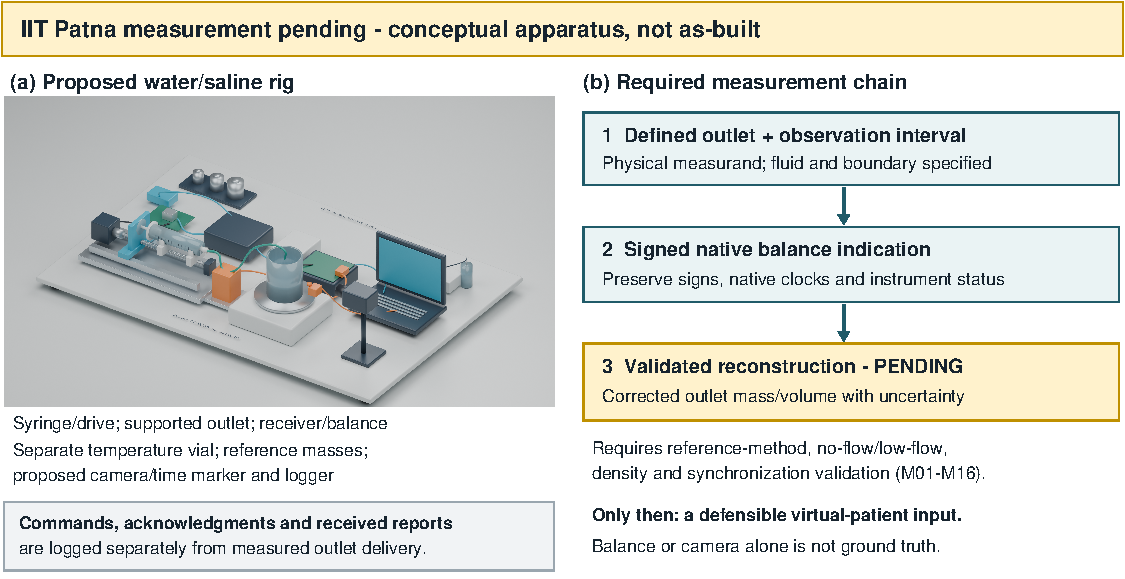
\includegraphics[width=\textwidth]{paper_figures/Figure3.pdf}\caption{IIT Patna measurement pending. Left: conceptual water/saline rig, not an as-built apparatus; components remain unselected. Right: proposed evidence chain from a defined outlet through signed native indications to a validated reconstruction with uncertainty. Commands and reports remain separate records. Balance and camera observations are not automatically ground truth. M01--M16 identify the required laboratory evidence.}\label{fig:3}\end{figure*}

The initial experiment should validate the measurand before connecting
any reconstructed input to a virtual plant. Define the outlet, interval,
fluid and hydraulic boundary. Record signed native indications,
instrument status, calibration identifiers and original clocks.
Characterize evaporation, drift, buoyancy where material, tubing
contact, surface tension, vibration, settling and density/temperature
uncertainty. Select a reference method with a documented calibration
chain and independence assumptions. A camera can help locate events
without automatically becoming a flow standard.

For an illustrative corrected mass difference
\(\Delta m_c=m_{\mathrm{end}}-m_{\mathrm{start}}-c_{\mathrm{blank}}\)
and volume \(V=\Delta m_c/\rho\), uncertainty propagation must include
density, correction and covariance terms \cite{R09}. Shared drift or
calibration errors need not be independent. Negative corrected estimates
near zero may arise from measurement noise; summing only positive
increments produces an avoidable zero-flow bias. Reconstruction,
filtering, latency and uncertainty must be validated against the chosen
reference using no-flow and low-flow trials before a method is frozen.

Stopping requires separate times for the event, monitor decision,
electrical command and a predefined flow-cessation criterion. Outlet
passage, receiver arrival and balance settling are distinct. Post-stop
mass needs a fixed follow-up and uncertainty; power removal does not
automatically eliminate fluid motion. Restart testing must preserve
withheld delivery, outstanding-command behavior and
failed/absent-operator cases. Blank acquisition templates and an offline
file validator enforce record structure only; a successful file check is
not metrological validation.

\begin{tcolorbox}[breakable,colback=pendingbg,colframe=pendingborder,boxrule=.5pt,arc=0pt,left=4pt,right=4pt,top=4pt,bottom=4pt]\textbf{IIT Patna measurement pending --- replacement fields.} M01:
actual components/as-built record; M02: measurand/outlet; M03: traceable
balance calibration; M04: fluid temperature/density; M05:
environmental/no-flow corrections; M06: mechanical force isolation; M07:
independent reference method; M08: reconstruction and zero-flow bias;
M09: delivery accuracy/timing; M10: clock synchronization; M11:
stop-event chain; M12: post-stop flow; M13: stop-path common modes; M14:
nuisance alarms/misses; M15: restart/recovery; M16: locked trial design
and complete immutable records. Replace a field only with raw-record
identity, method/version, uncertainty, trial denominator and human
review.\end{tcolorbox}

\begin{table*}[!t]
\centering
\caption{IIT Patna physical results pending}
\label{tab:4}
\small
\setlength{\tabcolsep}{3pt}
\renewcommand{\arraystretch}{1.17}
\begin{tabularx}{\linewidth}{>{\raggedright\arraybackslash}p{0.21\linewidth}>{\raggedright\arraybackslash}p{0.27\linewidth}>{\raggedright\arraybackslash}p{0.11\linewidth}>{\raggedright\arraybackslash}p{0.12\linewidth}>{\raggedright\arraybackslash}p{0.22\linewidth}}
\toprule
\textbf{Physical endpoint} & \textbf{Reference and unit} & \textbf{Result} & \textbf{Uncertainty} & \textbf{Status} \\
\midrule
\rowcolor{pendingbg}
Reconstructed outlet delivery & Validated reference; g or mL & Pending & Pending & IIT Patna measurement pending \\
\rowcolor{pendingbg}
Zero-flow cumulative bias & Matched blank; g or mL & Pending & Pending & IIT Patna measurement pending \\
\rowcolor{pendingbg}
Stop latency & Synchronized event chain; s & Pending & Pending & IIT Patna measurement pending \\
\rowcolor{pendingbg}
Post-stop delivery & Defined follow-up; g or mL & Pending & Pending & IIT Patna measurement pending \\
\rowcolor{pendingbg}
False-stop exposure & Benign trials; episodes/hour & Pending & Pending & IIT Patna measurement pending \\
\rowcolor{pendingbg}
Recovery deficit & Reference reconstruction; g or mL & Pending & Pending & IIT Patna measurement pending \\
\bottomrule
\end{tabularx}
\end{table*}

\section{Discussion and Limitations}

The main outcome is that complexity did not establish superiority. A
fuller score can accumulate evidence differently, trip later for abrupt
excess, or prolong authorization restrictions after recovery checks.
Because temporal aggregation and physiology corroboration change
together, the experiment cannot attribute a contrast solely to the twin.
The post-primary fasting supplement adds a delivery-CUSUM-only arm with
matched calibration exposure, while changing the operating regime; its
bounded result does not resolve the main meal-regime comparison. Varying
nuisance-stop budgets and reporting an excess/deficit frontier would be
more informative than choosing a favorable threshold after outcomes.

The forecast study similarly favors a qualified conclusion. A causal
selected baseline improved internal prediction relative to persistence,
while the mechanistic forecast usually did not. The physiology channel
still uses a corrected state estimator, but its selected future signal
is predominantly trend. Calling this outcome a validated mechanistic
digital twin would overstate the evidence. Near-bound parameters, proxy
inputs, interpolation, uneven record duration and previous test exposure
limit identifiability and generalization. Empirical residual coverage
also failed to control test alarm burden for many participants.

The Hovorka result reveals an applicability failure in this
implementation/regime, not a defect established in the original
publication. Published prior means, synthetic variation, added
observation lag and the selected controller were combined outside the
original fasting experiment. Negative endogenous production in clean
runs shows why a second equation family alone is insufficient evidence
of physiological robustness. Future validity work should begin with
declared operating regimes, equilibrium/response checks and pre-outcome
acceptance criteria. It should retain these failed-regime results rather
than replacing them with a favorable subgroup.

Several inference limits remain. Synthetic vectors are not patients;
repeated seeds do not enlarge the number of independent parameter units.
The fixed-request comparison estimates authorization effects for its
generated tapes, while the feedback sensitivity answers a different
question. The restricted conditions do not represent adaptive
adversaries or complete cybersecurity execution. The remaining local
measurement path and stop authority are assumed; common-mode compromise
can remove their usefulness. No glucose statistic establishes treatment
benefit, and no simulated research-U value should be interpreted as a
patient dose.

Physical follow-up should first establish reconstruction accuracy and
timing, then measure stop dynamics, then evaluate burden and recovery
with frozen analysis. This order matters because an apparently precise
comparator can be driven by biased delivery reconstruction. Water/saline
results would characterize an apparatus under tested conditions; they
would still not establish tissue absorption, clinical safety, deployment
readiness or institutional endorsement. Team review, authorship and
data-governance decisions remain required before submission.

\section{Conclusion}

GECO provides an explicit separation of delivery intent, authorization,
emission, observation and response in a reproducible offline study.
Causal forecast selection improved an internal retrospective baseline
comparison, but the shared-authority simulation did not establish a
fuller-detector advantage and exposed substantial physiological-domain
limitations. The next substantive step is validated delivery
reconstruction and measured stopping/recovery behavior on the proposed
rig, with IIT Patna measurements still pending.

\section*{Data, Code and Supplementary Material}

The working package retains the initial specification, amendments,
frozen calibration/configuration identities, complete attempt/failure
ledgers, participant metrics, paired synthetic contrasts and full
traces. Real-data and simulation results are separate. Supplementary
source access records distinguish full-text, partial and metadata-only
support. The HUPA and D1NAMO repository licenses and attribution
obligations apply to their material \cite{R14,R15}. Public deposition
and redistribution have not occurred as part of this work; the team must
select a release destination and confirm applicable permissions. No
proprietary similarity service or detector-based authorship
certification was used.

\section*{Author, Funding and AI-Use Statements --- Team Completion Required}

Author eligibility, names, affiliations, contributions, funding,
conflicts, ethics/data-governance determination and final approval are
pending the research team. No sample-paper author or institutional
endorsement is carried into this manuscript. IEEE authorship and
generated-content disclosure guidance will apply alongside the eventual
venue's instructions \cite{R10,R11,R12}.

Proposed disclosure for team confirmation: OpenAI Codex assisted with
literature organization and source checking, implementation and analysis
drafting, figure/media preparation, and manuscript drafting and
revision. Exact available tool/runtime information and verification
records are retained in the accompanying package; unavailable model
metadata are not inferred. Synthetic narration is identified in the
video. The team must state the actual human verification, corrections,
responsibility and final approval before submission. This pending
statement does not assert that those approvals have already occurred.
\bibliographystyle{IEEEtran}\bibliography{paper_references}
\end{document}